%============================================================
% CH1 · P3 · PROBLEM 2 — CHECK IF ARRAY IS SORTED AND ROTATED (LeetCode 1752)
%============================================================
\subsection{Problem 1.3.2: Check if Array Is Sorted and Rotated}
\problemlabel{1.3.2}{ssec:ch1-sorted-rotated}

\problemcard{1.3.2}{Check if Array Is Sorted and Rotated}{LeetCode 1752}{https://leetcode.com/problems/check-if-array-is-sorted-and-rotated/}{\exeasy\ \lc{Easy}}{Count the circular drops $a[i] > a[(i+1) \bmod n]$: at most one}

\subsubsection*{1. Problem statement}

Given an array \texttt{nums}, return \texttt{true} if it could have been obtained by taking an array sorted in \textbf{non-decreasing} order and rotating it by some number of positions (possibly zero), otherwise \texttt{false}. Duplicates are allowed. Rotating by $x$ positions means that the result $b$ satisfies $b[i] = a[(i + x) \bmod n]$ for the sorted array $a$.

\textbf{Constraints:} $1 \le n \le 100$, \; $1 \le \texttt{nums[i]} \le 100$.

\begin{table}[H]
\centering\small
\begin{tabular}{@{}lcl@{}}
\toprule
\textbf{nums} & \textbf{Output} & \textbf{Why} \\
\midrule
$[3,4,5,1,2]$ & \texttt{true} & $[1,2,3,4,5]$ rotated: reading from the 1 gives a sorted array \\
$[2,1,3,4]$ & \texttt{false} & no starting point gives a sorted array \\
$[1,2,3]$ & \texttt{true} & already sorted (rotation by 0) \\
\bottomrule
\end{tabular}
\end{table}

\begin{diagrambox}
\begin{tikzpicture}[x=1cm, y=1cm]
    \begin{scope}
        \dparray{a}{0}{}{3/acell, 4/acell, 5/aread, 1/aread, 2/acell}
        \draw[gcut] ([xshift=0.45cm, yshift=4mm]a2.north) -- ([xshift=0.45cm, yshift=-4mm]a2.south);
        \draw[back] ([yshift=-1mm]a4.south) to[bend left=25] node[lbl, below]{$2 \le 3$} ([yshift=-1mm]a0.south);
        \node[font=\scriptsize\bfseries] at (2.25,1.0) {Sample 1: one drop ($5 > 1$) \yes};
    \end{scope}
    \begin{scope}[xshift=6.3cm]
        \dparray{b}{0}{}{2/aread, 1/aread, 3/acell, 4/aread}
        \draw[gcut] ([xshift=0.45cm, yshift=4mm]b0.north) -- ([xshift=0.45cm, yshift=-4mm]b0.south);
        \draw[dep, warningred] ([yshift=-1mm]b3.south) to[bend left=25] node[lbl, below, text=warningred]{$4 > 2$} ([yshift=-1mm]b0.south);
        \node[font=\scriptsize\bfseries] at (1.8,1.0) {Sample 2: two drops \no};
    \end{scope}
    \begin{scope}[xshift=11.1cm]
        \dparray{c}{0}{}{1/acell, 2/acell, 3/acell}
        \draw[back] ([yshift=-1mm]c2.south) to[bend left=30] node[lbl, below, text=warningred]{$3 > 1$} ([yshift=-1mm]c0.south);
        \node[font=\scriptsize\bfseries] at (1.35,1.0) {Sample 3: one drop \yes};
    \end{scope}
\end{tikzpicture}
\figcap{The three official examples, with the wrap-around pair drawn as an arc from the last cell back to the first. Red dashed lines mark a drop between neighbours.}
\end{diagrambox}

\subsubsection*{2. The problem model}
\begin{modelbox}[Problem Model --- Sorted and Rotated]
\renewcommand{\arraystretch}{1.35}
\begin{tabularx}{\linewidth}{@{}>{\bfseries}l X@{}}
Input & an array $a[0..n-1]$ of small positive integers, duplicates allowed \\
Computed & a yes/no answer: does some start index $s$ make $a[s], a[s+1], \dots, a[n-1], a[0], \dots, a[s-1]$ non-decreasing? \\
Objects & the $n$ rotations of $a$ (equivalently, the $n$ \emph{circular} neighbour pairs $(a[i], a[(i+1) \bmod n])$) \\
Size & $n \le 100$: even $\bigO{n^2} = 10^4$ is instant; the interesting goal is a one-pass $\bigO{n}$, $\bigO{1}$-memory test \\
\end{tabularx}
\end{modelbox}

\begin{diagrambox}
\begin{tikzpicture}[x=1cm, y=1cm]
    \foreach \v/\i in {3/0, 4/1, 5/2, 1/3, 2/4}{
        \pgfmathsetmacro{\ang}{90-72*\i}
        \node[gv, minimum size=8mm] (r\i) at (\ang:1.4) {\v};
        \node[font=\scriptsize\color{darkgray}] at (\ang:2.05) {\i};
    }
    \foreach \i/\j in {0/1, 1/2, 3/4, 4/0}{ \draw[gde, draw=successgreen, line width=1.1pt] (r\i) -- (r\j); }
    \draw[gde, draw=warningred, line width=1.4pt, dashed] (r2) -- (r3);
    \node[note, anchor=west, text width=6.3cm, align=left] at (2.8,0.2)
        {Put the array on a circle. A rotation only changes \emph{where we start reading}; the circular neighbour pairs never change. Green arrows go up or stay level, the red one goes down.\\[3pt]
        A non-decreasing reading of all $n$ values exists $\iff$ we can start right after the only red arrow $\iff$ there is \textbf{at most one} red arrow.};
\end{tikzpicture}
\figcap{The model: a cyclic sequence with $n$ neighbour pairs (indices outside, values inside), here Sample 1.}
\end{diagrambox}

\subsubsection*{3. Key observations}

\begin{itemize}[leftmargin=*]
    \item \textbf{Rotations preserve the circle.} All $n$ rotations of $a$ have the same set of circular neighbour pairs $(a[i], a[(i+1) \bmod n])$. A sorted array has \emph{no} drop among its $n-1$ linear pairs; its circular pair (last, first) may or may not be a drop. So a rotated sorted array has at most one circular drop.
    \item \textbf{Tempting wrong idea 1 --- count only linear drops.} $[2,1,3,4]$ has a single linear drop ($2 > 1$) but the circular pair $(4, 2)$ is a second drop: the answer is \texttt{false}. The wrap-around pair must be counted.
    \item \textbf{Tempting wrong idea 2 --- start at the minimum.} ``Find the smallest value and check that reading from it is sorted'' fails with duplicates: in $[1,2,1,1]$ (a rotation of $[1,1,1,2]$) the first minimum is at index 0, and reading from there gives $1,2,1,1$ --- not sorted, so the idea answers \texttt{false}, but the answer is \texttt{true} (start at index 2).
    \item \textbf{Tempting wrong idea 3 --- treat equal neighbours as drops.} With $\ge$ instead of $>$, $[1,1,1]$ has three ``drops'' and would be rejected, though it is sorted.
\end{itemize}

\begin{diagrambox}
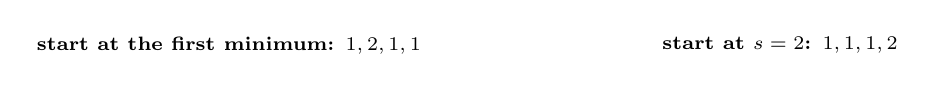
\begin{tikzpicture}[x=1cm, y=1cm]
    \begin{scope}
        \dparray{m}{0}{}{1/aread, 2/acell, 1/acell, 1/acell}
        \aptr{m0}{first min}{accentorange}
        \node[font=\scriptsize\bfseries] at (1.8,0.95) {start at the first minimum: $1,2,1,1$ \no};
    \end{scope}
    \begin{scope}[xshift=7cm]
        \dparray{o}{0}{}{1/acell, 2/acell, 1/akeep, 1/akeep}
        \aptr{o2}{start after the drop}{successgreen}
        \node[font=\scriptsize\bfseries] at (1.8,0.95) {start at $s = 2$: $1,1,1,2$ \yes};
    \end{scope}
\end{tikzpicture}
\figcap{Counter-example to ``start at the minimum'': with duplicates the right start is the cell after the drop, not the first copy of the minimum.}
\end{diagrambox}

\subsubsection*{4. Approaches}

\begin{bruteforcebox}
\textbf{Idea.} Try every start $s$ (``undo'' every possible rotation) and check whether the circular reading from $s$ is non-decreasing.
\begin{lstlisting}[style=cpp]
#include <bits/stdc++.h>
using namespace std;

class Solution {
public:
    bool check(vector<int>& nums) {
        int n = nums.size();
        for (int s = 0; s < n; s++) {          // try every start = undo every rotation
            bool ok = true;
            for (int j = 0; j + 1 < n; j++)
                if (nums[(s + j) % n] > nums[(s + j + 1) % n]) { ok = false; break; }
            if (ok) return true;
        }
        return false;
    }
};

int main() {                                   // input: n, then the n values
    int n;
    if (!(cin >> n)) return 0;
    vector<int> a(n);
    for (auto& x : a) cin >> x;
    cout << (Solution().check(a) ? "true" : "false") << "\n";
}
\end{lstlisting}
\begin{complexitybox}
\textbf{Time:} $\bigO{n^2}$ --- $10^4$ steps for $n = 100$, so it is \ac{} here; it would be too slow for $n = 10^5$ (the variants). \textbf{Space:} $\bigO{1}$ (indices mod $n$ instead of a rotated copy).
\end{complexitybox}
\end{bruteforcebox}

\begin{algorithmbox}
\textbf{Idea.} Count the circular drops: indices $i$ with $a[i] > a[(i+1) \bmod n]$. Answer \texttt{true} iff there are at most one.
\begin{lstlisting}[style=cpp]
#include <bits/stdc++.h>
using namespace std;

class Solution {
public:
    bool check(vector<int>& nums) {
        int n = nums.size(), drops = 0;
        for (int i = 0; i < n; i++)
            if (nums[i] > nums[(i + 1) % n])   // the pair (n-1, 0) is checked too
                drops++;
        return drops <= 1;
    }
};

int main() {                                   // input: n, then the n values
    int n;
    if (!(cin >> n)) return 0;
    vector<int> a(n);
    for (auto& x : a) cin >> x;
    cout << (Solution().check(a) ? "true" : "false") << "\n";
}
\end{lstlisting}
\begin{complexitybox}
\textbf{Time:} $\bigO{n}$ --- one pass over the $n$ circular pairs. \textbf{Space:} $\bigO{1}$. \textbf{Verdict:} \ac{}.
\end{complexitybox}
\end{algorithmbox}

\begin{invariantbox}[Why ``at most one circular drop'' is the exact test]
\textbf{($\Rightarrow$)} Let $b$ be non-decreasing and $a[i] = b[(i + x) \bmod n]$. The circular pairs of $a$ are the circular pairs of $b$, only listed from another start. Among the pairs of $b$, the $n-1$ linear ones $(b[j], b[j+1])$ are not drops, so only $(b[n-1], b[0])$ can be one: at most one drop.

\textbf{($\Leftarrow$)} If there is no drop, all values are equal around the circle (a cycle of $\le$ that returns to its start forces equality), and $a$ itself is sorted. If there is exactly one drop, at index $d$, read from $s = (d+1) \bmod n$: the $n-1$ pairs met along the way are all circular pairs except the one at $d$, so none is a drop, and the reading is non-decreasing. Hence $a$ is that sorted array rotated. \hfill$\blacksquare$

Note $n = 1$: the only pair is $(a[0], a[0])$, not a drop $\Rightarrow$ \texttt{true}.
\end{invariantbox}

\begin{alternativebox}
\textbf{Look for a sorted window in the doubled array.} Every rotation is a window of length $n$ in $a\,a$ (Tool~5 of the theory). Walk through $aa$ --- without building it, using index $j \bmod n$ --- and keep the length of the current non-decreasing run. The answer is \texttt{true} as soon as a run reaches length $n$.
\begin{lstlisting}[style=cpp]
#include <bits/stdc++.h>
using namespace std;

class Solution {
public:
    bool check(vector<int>& nums) {
        int n = nums.size();
        int run = 1;                              // length of the current non-decreasing run
        for (int j = 1; j < 2 * n; j++) {         // walk over nums + nums without building it
            if (nums[(j - 1) % n] <= nums[j % n]) run++;
            else run = 1;
            if (run >= n) return true;            // a sorted window of length n exists
        }
        return false;                             // (n = 1 already returned true)
    }
};

int main() {                                      // input: n, then the n values
    int n;
    if (!(cin >> n)) return 0;
    vector<int> a(n);
    for (auto& x : a) cin >> x;
    cout << (Solution().check(a) ? "true" : "false") << "\n";
}
\end{lstlisting}
Still $\bigO{n}$ time and $\bigO{1}$ memory, and it \emph{finds} the start: the window ends at $j$, so it begins at $(j - n + 1) \bmod n$. This form generalises to ``does some rotation satisfy a property that is checked pair by pair'', where counting drops has no direct analogue.

\begin{diagrambox}
\begin{tikzpicture}[x=1cm, y=1cm]
    \dparray{d}{0}{$a\,a$}{3/acell, 4/acell, 5/acell, 1/awin, 2/awin, 3/awin, 4/awin, 5/awin, 1/aout, 2/aout}
    \foreach \r [count=\j from 1] in {2,3,1,2,3,4,5}{ \node[font=\scriptsize\bfseries, text=deepblue] at (0.45+\j*0.9,0.75) {\r}; }
    \node[rowlabel, font=\scriptsize\color{deepblue}] at (-0.15,0.75) {run};
    \arange{d3}{d7}{run reaches $n = 5$ at $j = 7$: start $s = 3$}{memoorange}
\end{tikzpicture}
\figcap{Sample 1: the run length (blue) after each step $j$; the walk stops at $j = 7$ without looking at the last two cells.}
\end{diagrambox}
\end{alternativebox}

\begin{tricksbox}
\begin{itemize}[leftmargin=*]
    \item \textbf{Early exit:} return \texttt{false} as soon as the second drop is found.
    \item \textbf{Strictly increasing variant:} if the original array must be \emph{strictly} increasing, a drop is $a[i] \ge a[(i+1) \bmod n]$ and the test stays ``at most one drop'' (for $n = 1$ the single pair $(a[0], a[0])$ is then the one allowed drop).
    \item \textbf{Avoid \texttt{\%} in the loop:} check the $n-1$ linear pairs, then add the pair $(a[n-1], a[0])$ separately; the result is the same.
\end{itemize}
\end{tricksbox}

\subsubsection*{5. Trace}

\begin{tracebox}[{Sample 1 $[3,4,5,1,2]$ and Sample 2 $[2,1,3,4]$}]
\centering
\begin{tikzpicture}[x=1cm, y=1cm]
    \dparray{p}{1.4}{Sample 1}{3/acell, 4/acell, 5/aread, 1/acell, 2/acell}
    \aptr{p2}{drop 1}{warningred}
    \draw[back] ([yshift=1mm]p4.north) to[bend right=22] node[lbl, above]{$2 \le 3$: no drop} ([yshift=1mm]p0.north);
    \dparray{q}{-1.4}{Sample 2}{2/aread, 1/acell, 3/acell, 4/aread}
    \aptr{q0}{drop 1}{warningred}
    \aptr{q3}{drop 2}{warningred}
    \draw[dep, warningred] ([yshift=1mm]q3.north) to[bend right=25] node[lbl, above, text=warningred]{$4 > 2$} ([yshift=1mm]q0.north);
    \node[note, anchor=west, text width=4.3cm, align=left] at (5.4,1.4) {one drop, at $i = 2$ ($5 > 1$) $\Rightarrow$ \texttt{true}; the sorted reading starts at $i = 3$};
    \node[note, anchor=west, text width=4.3cm, align=left] at (5.4,-1.4) {drops at $i = 0$ ($2 > 1$) and at the seam $i = 3$ ($4 > 2$) $\Rightarrow$ \texttt{false}};
\end{tikzpicture}
\figcap{Red pointers mark the indices $i$ where $a[i] > a[(i+1) \bmod n]$.}

\medskip
\small
\begin{tabular}{@{}c|cccc|cccc@{}}
\toprule
 & \multicolumn{4}{c|}{\textbf{Sample 1}} & \multicolumn{4}{c}{\textbf{Sample 2}} \\
$i$ & $a[i]$ & $a[(i+1) \bmod n]$ & drop? & \texttt{drops} & $a[i]$ & $a[(i+1) \bmod n]$ & drop? & \texttt{drops} \\
\midrule
0 & 3 & 4 & no & 0 & 2 & 1 & \textbf{yes} & 1 \\
1 & 4 & 5 & no & 0 & 1 & 3 & no & 1 \\
2 & 5 & 1 & \textbf{yes} & 1 & 3 & 4 & no & 1 \\
3 & 1 & 2 & no & 1 & 4 & 2 & \textbf{yes} & 2 \\
4 & 2 & 3 & no & 1 & \multicolumn{4}{c}{---} \\
\midrule
 & \multicolumn{4}{c|}{$1 \le 1 \Rightarrow$ \texttt{true}} & \multicolumn{4}{c}{$2 > 1 \Rightarrow$ \texttt{false}} \\
\bottomrule
\end{tabular}
\end{tracebox}

\begin{tracebox}[{Duplicates: $[1,2,1,1]$}]
\centering
\begin{tikzpicture}[x=1cm, y=1cm]
    \dparray{u}{0}{}{1/acell, 2/aread, 1/acell, 1/acell}
    \aptr{u1}{only drop}{warningred}
    \draw[back] ([yshift=1mm]u3.north) to[bend right=25] node[lbl, above]{$1 \le 1$} ([yshift=1mm]u0.north);
    \node[note, anchor=west, text width=6.4cm, align=left] at (4.0,0) {pairs: $(1,2)$ ok, $(2,1)$ drop, $(1,1)$ ok, $(1,1)$ ok (the seam). One drop $\Rightarrow$ \texttt{true}; the sorted reading $1,1,1,2$ starts at $i = 2$. The doubled-array walk reaches run length 4 at $j = 5$, i.e.\ the window starting at $(5-4+1) \bmod 4 = 2$.};
\end{tikzpicture}
\figcap{Equal neighbours are not drops, so duplicates need no special handling.}
\end{tracebox}

\subsubsection*{6. Test suite}

\begin{testbox}
\centering\small
\begin{tabular}{@{}lll@{}}
\toprule
\textbf{nums} & \textbf{Why it is interesting} & \textbf{Expected} \\
\midrule
$[3,4,5,1,2]$ & official Sample 1 & \texttt{true} \\
$[2,1,3,4]$ & official Sample 2: one linear drop + the seam & \texttt{false} \\
$[1,2,3]$ & official Sample 3: rotation by 0 & \texttt{true} \\
$[7]$ & $n = 1$ & \texttt{true} \\
$[5,5,5,5]$ & all equal: zero drops & \texttt{true} \\
$[1,2,1,1]$ & duplicates; ``start at the minimum'' fails & \texttt{true} \\
$[2,2,1,2,1]$ & two drops hidden among duplicates & \texttt{false} \\
$[3,2,1]$ & reversed sorted array: two drops & \texttt{false} \\
\bottomrule
\end{tabular}

\medskip
The three programs agree on the official samples and on 500 random arrays ($n \le 7$, values $1..4$, half of them rotated sorted arrays, some with one value disturbed).
\end{testbox}

\subsubsection*{7. Common mistakes}

\begin{warningbox}[Mistake 1 --- forgetting the seam]
\begin{lstlisting}[style=snippet]
for (int i = 0; i + 1 < n; i++) if (a[i] > a[i + 1]) drops++;   // WRONG: [2,1,3,4] -> true
for (int i = 0; i < n; i++) if (a[i] > a[(i + 1) % n]) drops++;  // RIGHT
\end{lstlisting}
\end{warningbox}

\begin{warningbox}[Mistake 2 --- $\ge$ instead of $>$]
The original array is \emph{non-decreasing}; equal neighbours are allowed. Counting $a[i] \ge a[i+1]$ rejects $[1,1,1]$ and $[2,2,3]$.
\end{warningbox}

\begin{warningbox}[Mistake 3 --- ``exactly one drop'']
\texttt{return drops == 1;} rejects arrays with zero drops. That happens only when all values are equal (any other sorted array has the seam drop), e.g.\ $[4,4,4]$, which must return \texttt{true}.
\end{warningbox}

\begin{warningbox}[Mistake 4 --- starting from the minimum]
Locating the minimum and checking from its first occurrence breaks on duplicates ($[1,2,1,1]$); locating it from the last occurrence breaks on $[2,1,1]$ (reading $1,2,1$). The drop is the reliable landmark.
\end{warningbox}

\subsubsection*{8. Takeaways}

\begin{itemize}[leftmargin=*]
    \item A rotation does not change the circle: properties of ``some rotation'' are often properties of the circular neighbour pairs.
    \item A rotated sorted array has at most one circular drop, and the sorted reading starts right after it.
    \item The doubled array $aa$ turns ``some rotation has property $P$'' into ``some window of length $n$ has property $P$'' --- index it with $j \bmod n$.
    \item With duplicates, anchor on the drop, never on the position of the minimum.
\end{itemize}

\begin{variantsbox}
\variant{Minimum Right Shifts to Sort the Array}{\exeasy\ \lc{Easy}\ \varlink{Minimum Right Shifts to Sort the Array}{LeetCode 2855}{https://leetcode.com/problems/minimum-right-shifts-to-sort-the-array/}}
  {distinct values; return the minimum number of right shifts that sorts the array, or $-1$.}
  {model: zero drops $\Rightarrow 0$; two or more $\Rightarrow -1$; one drop at $d$: the sorted reading starts at $d+1$.}
  {algorithm: the same drop count; answer $n - 1 - d$ for the single drop. Samples $\to 2, 0, -1$; checked against shifting $n$ times.}
\variant{Bazoka and Mocha's Array}{\exeasy\ \cf{800}\ \varlink{Bazoka and Mocha's Array}{Codeforces 1975A}{https://codeforces.com/problemset/problem/1975/A}}
  {an operation splits the array into a prefix and a suffix and swaps them; can it become non-decreasing?}
  {model: prefix--suffix swaps are rotations, so the question is exactly ``is it a rotated sorted array?''.}
  {algorithm: the circular drop count per test case ($n \le 50$); sample $\to$ No, Yes, Yes.}
\variant{Rotate String}{\exeasy\ \lc{Easy}\ \varlink{Rotate String}{LeetCode 796}{https://leetcode.com/problems/rotate-string/}}
  {given two strings $s$ and $g$, can repeated ``move the first character to the end'' turn $s$ into $g$?}
  {model: is $g$ a rotation of $s$? $\iff |s| = |g|$ and $g$ is a window of $ss$ (Tool~5).}
  {algorithm: \texttt{s.size() == g.size() \&\& (s + s).find(g) != npos}, $\bigO{n^2}$ for $n \le 100$; samples $\to$ true, false.}
\variant{Sorted descending and rotated}{\varnone}
  {was the array obtained by rotating a \emph{non-increasing} array?}
  {model: mirror image: count circular \emph{rises} $a[i] < a[(i+1) \bmod n]$.}
  {algorithm: the same one pass with $<$; \texttt{true} iff at most one rise.}
\end{variantsbox}
